\documentclass[main]{subfiles}

\begin{document}
    \section{Функции от нескольких переменных}
    \Date{02.09.2019}
    \subsection{Основные определения}

    \begin{definition}
        $\rho: X * X \ra \R$ - метрика, если
        \begin{enumerate}
          \item $\rho(x,y) \geqslant 0$, $\rho(x,y)=0 \Lra x=y$
          \item $\rho(x,y)=\rho(y,x)$
          \item $\rho(x,y) \leqslant \rho(x,z)+\rho(z,y)$

          $(X,\rho)$ - метрическое пространство
      \end{enumerate}
    \end{definition}

    \begin{examples}
        \begin{enumerate}
            \item $\R$ $\rho(x,y)=|x-y|$
            \item $x \neq \varnothing$ $\rho(x,y)=
                \begin{cases}
                    1, \q x \neq y\\
                    0, \q x=y
                \end{cases}$
            \item $\R^n$, $n \geqslant 1$ $\rho(x,y)=\sqrt{(x_1-y_1)^2+...+(x_n-y_n)^2}$,

            где $x=(x_1,...,x_n)$ $y=(y_1,...,y_n)$
        \end{enumerate}
    \end{examples}

    \begin{definition}
        $\rho_1, \rho_2: X*X \ra \R$ - метрики, тогда $\rho_1, \rho_2$ - эквивалентны, если

        (они задают одну топологию) $c_1 \rho_1 (x,y) \leqslant \rho_2 (x,y) \leqslant c_2 \rho_1(x,y)$ для $c_1,c_2>0$ - $\const$
    \end{definition}

    \begin{example}
        $\R^2$ $\rho_1(x,y) = \sqrt{(x_1-y_1)^2 + (x_2-y_2)^2} \leqslant \sqrt{2 \rho_2^2(x,y)}$

        $\rho_2(x,y)=max(|x_1-y_1|, |x_2-y_2|)$ (упр.)

        $\frac{1}{\sqrt{2}} \rho_1(x,y) \leqslant \rho_2(x,y) \leqslant \rho_1(x,y)$

        Пусть $\rho_3(x,y)=(|x_1-y_1|^p+...|x-n-y_n|^p)^{\frac{1}{p}}$, $p \geqslant 1$

        Если $p \ra \infty$ $\rho_3 \ra \rho_2$

        $l_n^p=(\R^n,\rho_3)$ - пространство Лебега конечномерное

        (упр.) Д-ть, что все метрики эквивалентны $(\rho_1,\rho_2,\rho_3)$

        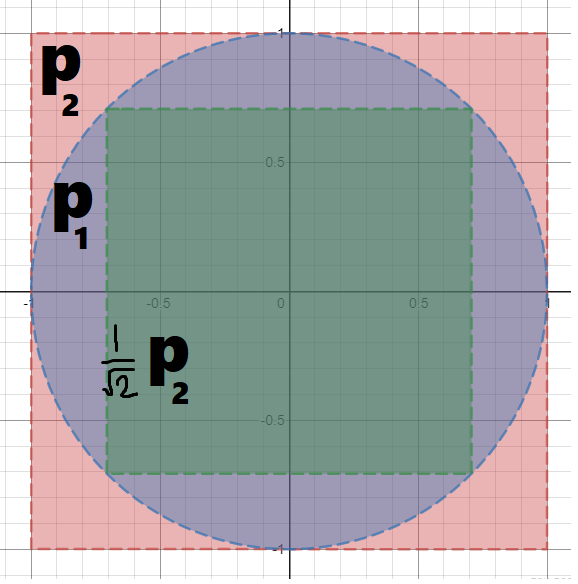
\includegraphics[scale=0.3]{pics/p1p2p3.png}
    \end{example}

    \begin{definition}
        $\rho: X*X \ra \R$ - метрика,

        Открытым шаром в X относительно метрики $\rho$ называется мн-во $B_r(x)=B(x,r)=\{y \in X: \rho(x,y) < r \}$

        Замкнутым шаром называется $\ol{B}_r(x)=\{y \in X: \rho(y,x) \leqslant r \}$

        Сферой называется $S_r(x)=\{y \in X: \rho(x,y)=r \}$
    \end{definition}

    \begin{upr}
        Замкнутый шар - не всегда замыкание шара (см. дискретную метрику)
    \end{upr}

    \begin{example}
        $l^p=\{ \{x_n\}_{n=1}^\infty: \sum\limits_{n=1}^\infty |x_n|^p < \infty \}$ $1 \leqslant p < \infty$

        $\rho(\{x_n\}_{n=1}^\infty, \{y_n\}_{n=1}^\infty) = (\sum\limits_{n=1}^\infty (x_n-y_n)^p)^{\frac{1}{p}}$

        $l^p$ - пр-во Лебега (последовательностей)
    \end{example}

    \begin{example}
        $C[0,1]$ - пр-во непр. функций

        $\rho(f,g)=\max\limits_{[0,1]} |f-g|$ - полна (любая фундаментальная последовательность сходится)

        $\rho_p(f,g)=(\int\limits_0^1 |f-g|^p dx)^{\frac{1}{p}}$ - не полная
    \end{example}

    \begin{definition}
        $(X, \rho)$ - метр. пр-во, $\{x_k\}_{k=1}^\infty \subset X$, $a \in X$ $x_k \ra a$ в пр-ве X по метрике $\rho$, если $\rho(x_n,a) \us{k \ra \infty}{\ra} 0$
    \end{definition}

    \begin{examples}
        $\R^2$ $M_k=(x_k, y_k)$ $P=(a,b)$ $M_k \ra P$ в евкл. метрике, т.е. $\rho(M_k,P)=\sqrt{(x_k-a)^2+(y_k-b)^2} \us{k \ra \infty}{\ra} 0 \Lra x_k \ra a,\ y_k \ra b$
    \end{examples}

    \begin{remark}
        Есть $\rho_1,\rho_2$ - экв. метрики, то $\rho_1(x_k,a) \ra 0 \Lra \rho_2(x_k,a) \ra 0$
    \end{remark}

    \begin{upr}
        $x_k \ra a,\ x_k \ra b \Ra a=b$

        ($\rho(a,b) \leqslant \rho(a, x_k) + \rho(x_k,b) \ra 0 \Ra \rho (a,b) \ra 0 \Ra a=b$)
    \end{upr}

    \begin{definition}
        $E \subset X$, $(X, \rho)$ - метр. пр-во, то $a \in X$ - т. сгущ. E, если

        $\forall \E \ \e x \in E: \rho(a,x) < \E$
    \end{definition}

    \begin{definition}
        $f:E \ra Y$ $(X, \rho)$, $(Y,d)$ - метр. пр-ва $(E \subset X)$, а - т. сгущ. E, $A \in Y$,

        тогда A - предел отображения f в точке а, если

        $f(x) \ra A$ при $x \in E \setminus \{a\}\ra a$\\
        (или $\forall \E>0 \q \e \delta>0: \rho(x,a)<\delta$ и $x \in E \subset \{a\}$, то $d(f(x),A) < \E)$\\
        Обозначение: $A=\lim\limits_{x \ra a} f(x)$ или $f(x) \ra A$ $x \ra a$
    \end{definition}

    \begin{remark}
        $A=\lim\limits_{x \ra a} f(x) \Lra \forall \E > 0 \ \e \delta>0: f(B_\delta(a) \setminus \{a\}) \subset B_\E (A)$
    \end{remark}
\end{document}
